\section{Photon Antibunching}\label{sec:photon-antibunching}
Remember that light can be classified according to its photon statistics. We have already used Young's experiment and the Mach--Zehnder interferometer to introduce the concept of first-order coherence (Eqn.~\ref{eqn:6-degree-of-first-order-coherence}):
\begin{equation}
g^{(1)}(\tau)=\frac{\langle E^*(t)\,E(t+\tau)\rangle}{\langle E^*(t)\,E(t)\rangle},
\end{equation}

which is useful for determining how monochromatic a source is and for estimating the coherence time or coherence length of the light. However, \hl{first-order coherence does not contain information about the actual statistical properties of the light field}. That information is carried by the \textbf{intensity fluctuations}.

Suppose that we perform two-time measurements in which many pairs of intensity readings are taken with a fixed time delay $\tau$. The average of the product of each pair of readings defines the \textbf{intensity correlation function}, which is the intensity analogue of the first-order field correlation function.

We are interested in measuring the coincidence rate:
\[
C(t,t+\tau)=\langle I(t)\,I(t+\tau)\rangle,
\]

where the two intensities are detected by two different detectors.

If the field is stationary, the average depends only on the time delay, so we can define the \textbf{second-order correlation function} as
\begin{equation}\label{eqn:10-second-order-correlation-function}
g^{(2)}(\tau)=
\frac{\langle I(t)\,I(t+\tau)\rangle}{\langle I(t)\rangle^2} =
\frac{\langle E^*(t)E^*(t+\tau)E(t)E(t+\tau)\rangle}{\langle E^*(t)E(t)\rangle^2}.
\end{equation}

For a classical stationary field, the normalized first-order correlation satisfies
\[
|g^{(1)}(\tau)|\le 1.
\]

If the intensity is constant, $I(t)=I(t+\tau)=I_0$, then
\[
g^{(2)}(\tau)=1.
\]

When $\tau = 0 \implies g^{(2)}(0) = \frac{\braket{I(t)^2}}{\braket{I(t)}^2}$ and for a sequence of N measurements taken at times $t_1,t_2,...t_N$ the averages are given by:
\[\braket{I(t)} = \frac{I(t_1)+...+I(t_N)}{N}\hspace{1cm}\braket{I(t)^2} = \frac{I^2(t_1)+...+I^2(t_N)}{N}\]

But according to \textbf{Cauchy inequality}: 
\begin{equation}\label{eqn:cauchy-inequality}
2\cdot I(t_1)\cdot I(t_2) \leq I^2(t_1)+I^2(t_2)
\end{equation}

it applies to any pair of time $t_i$ and hence to all cross terms in $\braket{I^2(t)}$, we obtain:
\[\braket{I^2(t)} \geq \braket{I(t)}^2 \implies g^{(2)}(0) = \frac{\braket{I(t)^2}}{\braket{I(t)}^2}\geq 1 \]

There is no way to establish an upper limit, so the allowed values are:
\[1 \leq g^{(2)}(0) < +\infty\]

For not-zero time delays, the positive nature of the intensity guarantees that:
\[0 \leq g^{(2)}(\tau) < +\infty\]

We can also obtain another result using the Cauchy inequality:
\begin{equation}\label{eqn:cauchy-inequality-2}
[I(t_1) I(t_1+\tau) + \dots + I(t_N) I(t_N+\tau)]^2 \leq 
\left[
    [I^2(t_1) + \dots + I^2(t_N)] [I^2(t_1+\tau) + \dots + I^2(t_N+\tau)]
\right]
\end{equation}

For a long series of measurements, the two series on the right hand side are equivalent and the square root of the previous equation leads to:
\[\braket{I(t) \cdot I(t+\tau)} \leq \braket{I(t)}^2\]
\[\implies g^{(2)}(\tau) = \frac{\braket{I(t)\cdot I(t+\tau)}}{\braket{I(t)}^2} \leq 1 \leq g^{(2)}(0) \]

\calloutinfo{%
So we obtain the \textbf{limits for classical light fields}:
\begin{equation}\label{eqn:10-classical-light-second-order-correlation}
g^{(2)}(\tau) < g^{(2)}(0) \hspace{1ex} \land \hspace{1ex}
1 \leq g^{(2)}(0) < +\infty, \hspace{1ex} \forall\tau \ne 0
\end{equation}

This means that, within classical optics, the \textbf{zero-delay correlation is the largest one}. A violation of this condition is a signature of quantum light.
}

We can now consider some important cases:
\begin{enumerate}
    \item \hl{For a perfectly coherent light field},
    \begin{equation}\label{eqn:10-coherent-light-second-order-correlation}
    g^{(2)}(\tau)=1 \qquad \forall\,\tau.
    \end{equation}
    This is the expected result for an ideal laser-like source with Poissonian photon statistics.

    \item \hl{For a light source made of a large number of independent emitters}, undergoing collisions and \emph{Doppler broadening}, the field is \emph{chaotic} and gaussian distributed. In this case the \textbf{Siegert relation} holds:
    \begin{equation}\label{eqn:10-siegert-relation}
    g^{(2)}(\tau)=1+|g^{(1)}(\tau)|^2
    \end{equation}

    and since
    \[
    0\le |g^{(1)}(\tau)|\le 1,
    \]

    one has
    \begin{equation}\label{eqn:10-chaotic-light-second-order-correlation}
    1\le g^{(2)}(\tau)\le 2.
    \end{equation}

    This is the typical bunching behavior of thermal light.

    \item \hl{For a source with a Lorentzian spectral profile}, such as a collision-broadened source,
    \[
    g^{(2)}(\tau)=1+e^{-2|\tau|/\tau_c},
    \]

    so that
    \[
    g^{(2)}(\tau)\to 1 \qquad \text{for } |\tau|\to\infty,
    \]

    and
    \[
    g^{(2)}(0)\to 2.
    \]
\end{enumerate}
\begin{figure}[H]
    \centering
    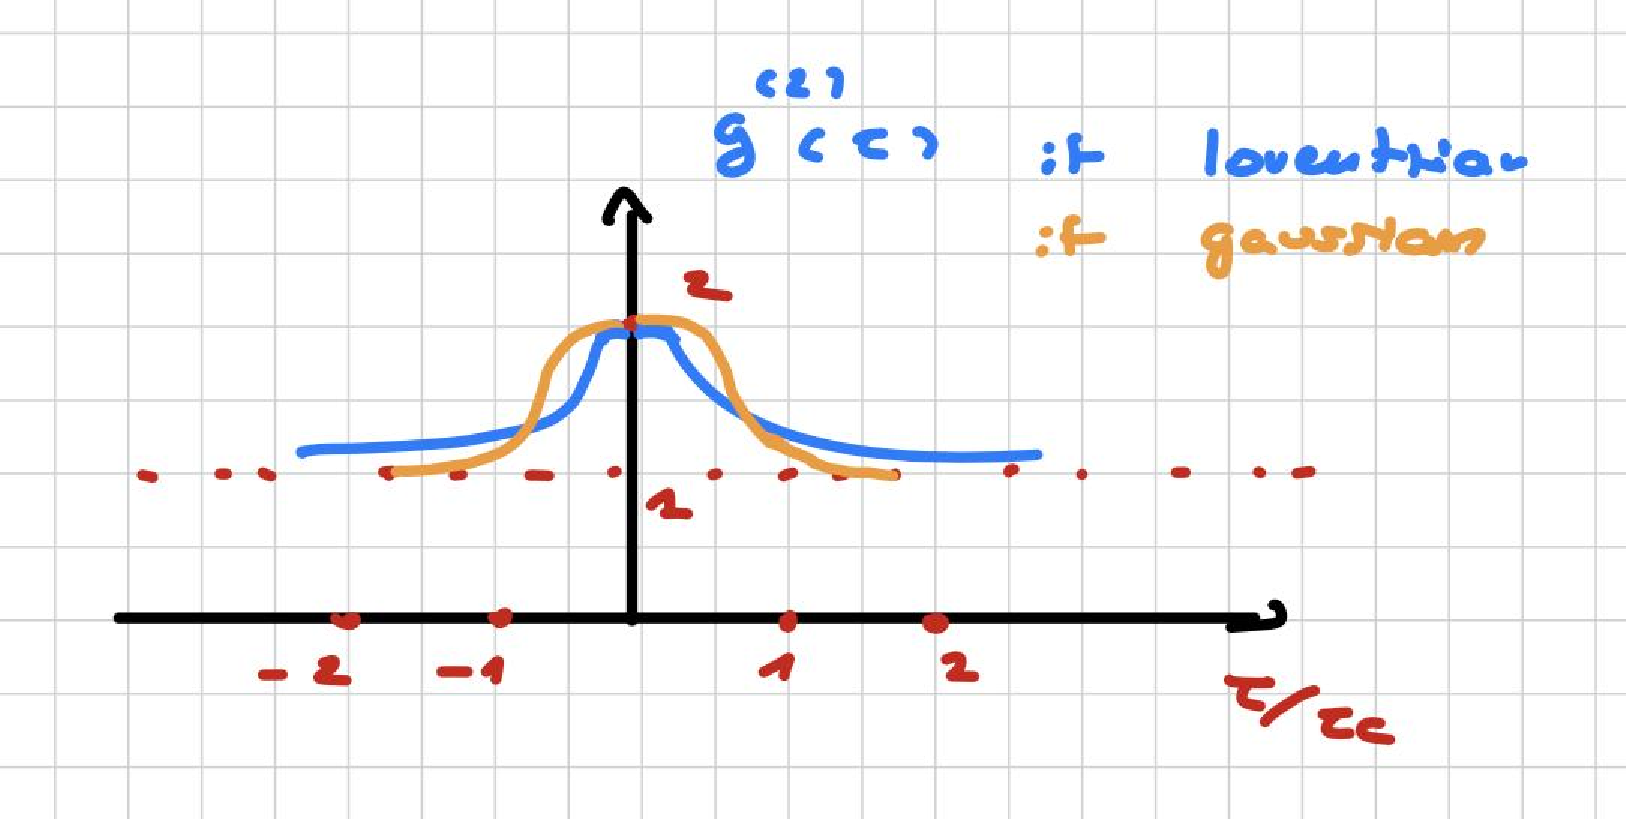
\includegraphics[width=0.6\linewidth]{images_in_pdf/10-/Grafico_52.pdf}
\end{figure}

The peak of $g^{(2)}(\tau)$ for $|\tau|<\tau_c$ is a manifestation of short-time intensity fluctuations. For $|\tau|\gg\tau_c$, the two intensities become essentially uncorrelated and the second-order coherence approaches unity.

\subsection{Second-order correlation measurement: Hanbury Brown and Twiss}

The famous \textbf{Hanbury Brown and Twiss (HBT)} experiment introduced a new type of correlation measurement. While a Mach--Zehnder interferometer is sensitive to first-order coherence and therefore to phase correlations of the electric field, the HBT setup probes intensity correlations and second-order coherence.
\begin{figure}[H]
    \centering
    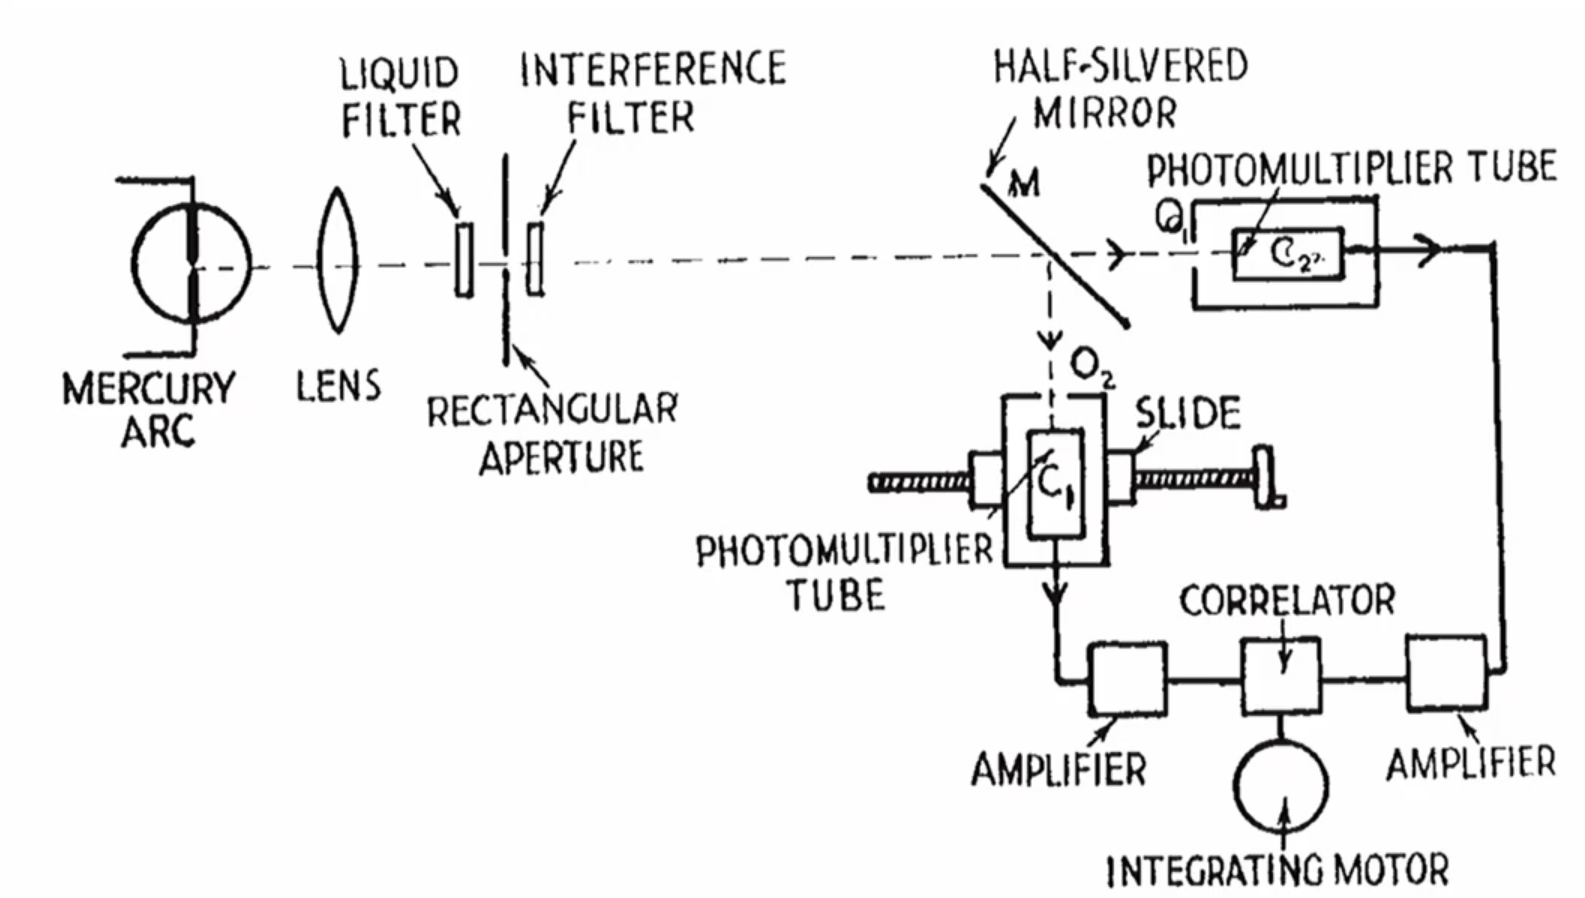
\includegraphics[width=0.6\linewidth]{images_in_png/Grafico_52a.png}
\end{figure}
\begin{itemize}
    \item As a source, Hanbury Brown and Twiss used a mercury lamp emitting at $\lambda = \qty{435.8}{\nano\meter}$;
    \item The signal passes through lenses and filters, so that it becomes collimated and spectrally selected;
    \item It then reaches a $50:50$ beam splitter, and each output is sent to a photomultiplier tube;
    \item The two output signals are amplified and fed into a correlator, which measures the average product of the intensity fluctuations over long observation times.
\end{itemize}
We assume that the detectors are placed symmetrically, so that the two optical paths are identical. Then
\[
I_1(t)=I_2(t)\equiv I(t),
\]
with
\[
I(t)=\langle I(t)\rangle+\Delta I(t).
\]
Here $2I(t)$ is the total intensity incident on the beam splitter, while $\Delta I(t)$ represents the fluctuations around the mean value. The output of the correlator is proportional to
\[
\langle \Delta I(t)\,\Delta I(t+\tau)\rangle.
\]
At $\tau=0$, the two paths are identical and
\[
\langle \Delta I^2(t)\rangle\neq 0,
\]
while
\[
\langle \Delta I(t)\rangle=0.
\]
When $|\tau|\gg\tau_c$, the fluctuations become uncorrelated, so
\[
\langle \Delta I(t)\,\Delta I(t+\tau)\rangle \to 0.
\]
Therefore, measuring the output as a function of $\tau$ provides information about the coherence time $\tau_c$. In the original HBT interferometer, varying the detector separation was used to probe the spatial coherence of the source rather than its temporal coherence.

\subsection{Bunched and anti-bunched light in HBT}
Here a simplified scheme of the HBT interferometer is presented:
\begin{figure}[H]
    \centering
    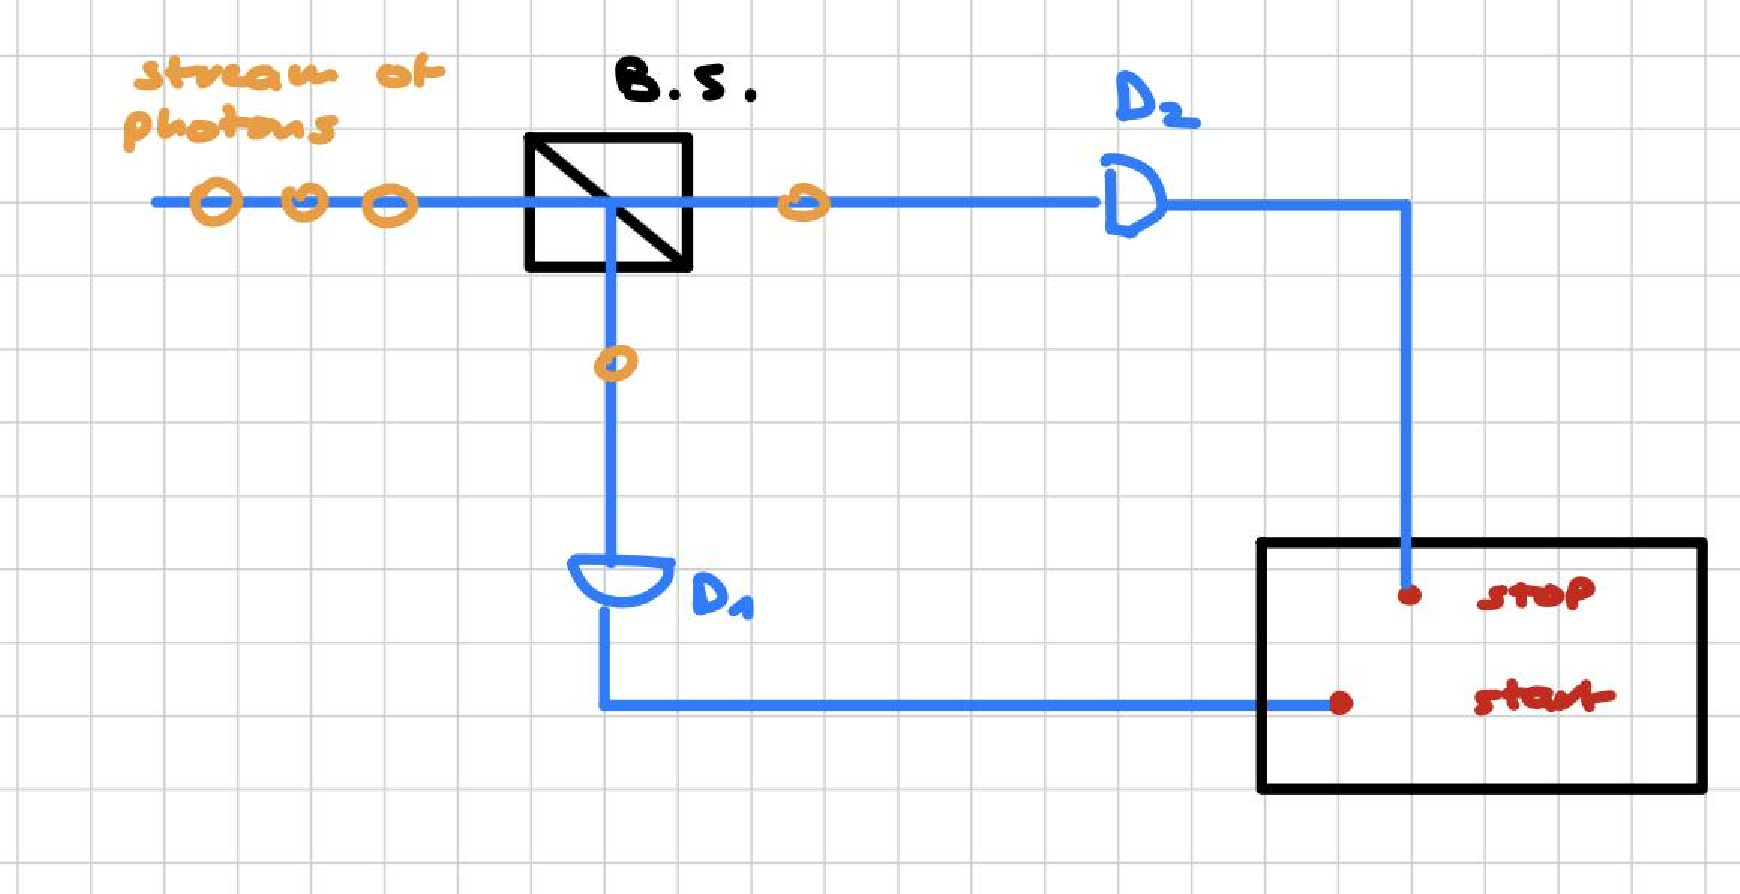
\includegraphics[width=0.6\linewidth]{images_in_pdf/10-/Grafico_53.pdf}
\end{figure}

The light beam is sent to a beam splitter. The reflected part reaches detector $D_1$ and starts the timing electronics, while the transmitted part reaches detector $D_2$ and provides the stop signal. In this way, we count the number of coincidence events while measuring the time delay between the two detectors.\\
The second-order correlation function $g^{(2)}(\tau)$ is proportional to the conditional probability of detecting a second photon at $D_2$ at time $t=\tau$, given that another photon has been detected at $D_1$ at time $t=0$.\\
The Hanbury Brown and Twiss interferometer provides a direct measurement of $g^{(2)}(\tau)$. If we define $n_i(t)$ as the number of counts registered by detector $D_i$ at time $t$, then:
\begin{equation}\label{eqn:10-second-order-correlation-function-photon-counting}
g^{(2)}(\tau)=\frac{\langle n_1(t)\,n_2(t+\tau)\rangle}{\langle n_1(t)\rangle\,\langle n_2(t+\tau)\rangle}.
\end{equation}

\hl{Since $n_i \propto I$}, we can build a histogram that shows the number of coincidence events observed within a given time interval:
\begin{figure}[H]
    \centering
    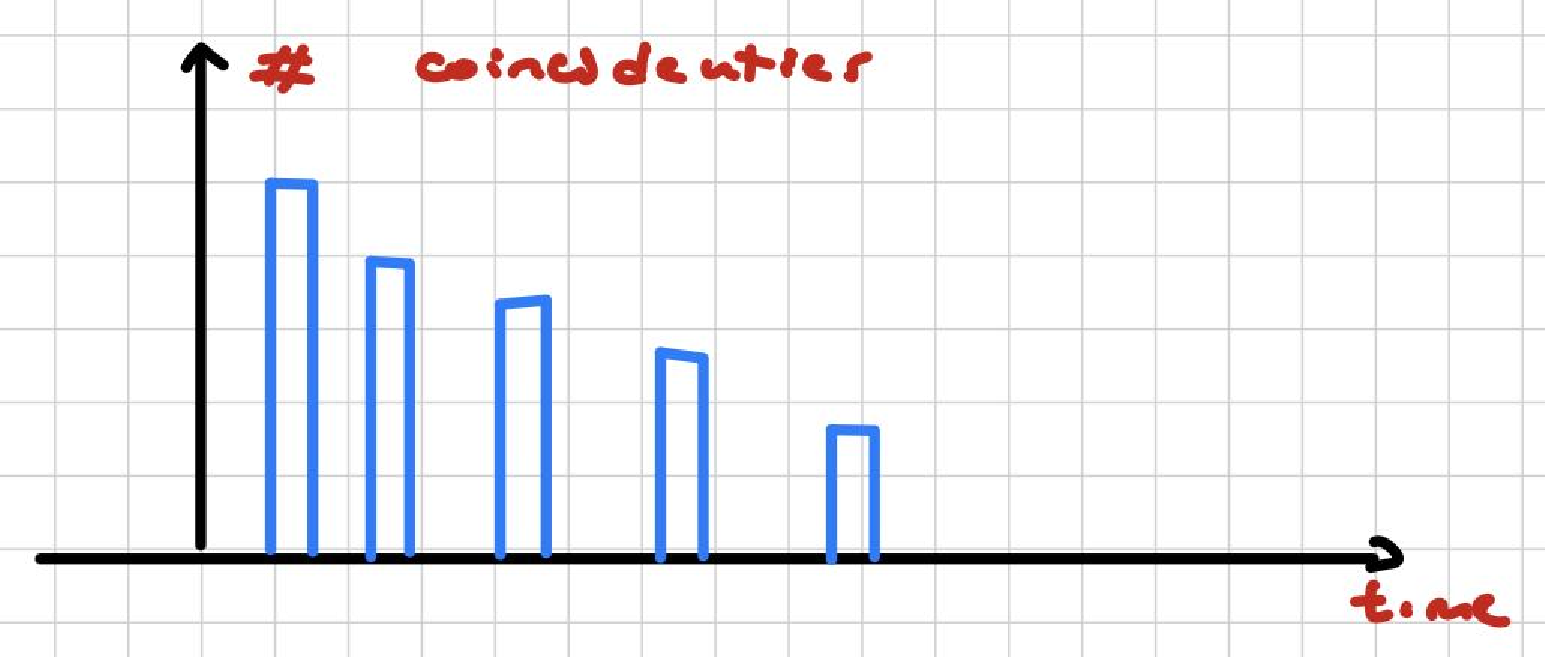
\includegraphics[width=0.6\linewidth]{images_in_pdf/10-/Grafico_54.pdf}
\end{figure}

\calloutinfo{%
\begin{itemize}
    \item \textbf{If we are dealing with a stream of well-separated photons}, there is a $50\%$ probability that one photon is reflected to $D_1$ and starts the timer, but the same photon cannot also generate a stop signal at $D_2$. Therefore, ideally, we expect no coincidences at $\tau=0$. The next photon may later be transmitted to $D_2$ and stop the timer, so coincidence events appear only at nonzero delays. This means that the conditional probability of detecting a second photon immediately after the first one is suppressed, and thus
    \begin{equation}\label{eqn:10-photon-antibunching}
    g^{(2)}(0) < g^{(2)}(\tau),
    \end{equation}

    which is a signature of nonclassical light. This is the case of \textbf{anti-bunched light}, namely a stream of individual photons separated in time by emission dynamics rather than by classical randomness.

    \item\textbf{On the other hand, if many photons arrive in groups}, then both detectors have a high probability of clicking at nearly the same time. In that case, the coincidence histogram shows a large peak around $\tau=0$, and the correlation function decreases as $\tau$ increases because the probability of detecting two photons from the same bunch becomes smaller. This is the typical behavior of \textbf{bunched light}, which is characteristic of chaotic classical sources.
\end{itemize}
}

\subsection{Light classification in terms of $g^{(2)}(0)$}

At the end, we obtain a way to classify light according to the value of $g^{(2)}(0)$:
\begin{enumerate}
    \item \textbf{Coherent light:} Poissonian statistics with random time intervals between photons, where
    \[
    g^{(2)}(\tau)=1 \qquad \forall\,\tau.
    \]

    The probability of obtaining a stop pulse is the same at any delay, and in particular
    \[
    g^{(2)}(0)=1.
    \]

    \item \textbf{Bunched light:}
    \begin{figure}[H]
        \centering
        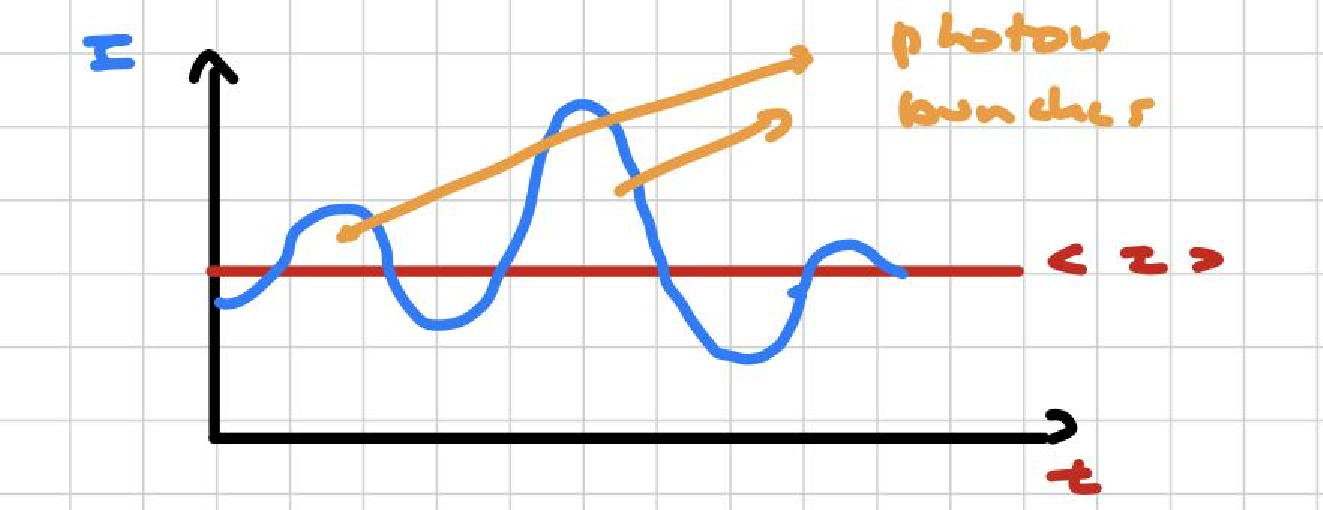
\includegraphics[width=0.6\linewidth]{images_in_pdf/10-/Grafico_55.pdf}
    \end{figure}
    \[
    g^{(2)}(\tau)=
    \begin{cases}
        \text{large for small } \tau,\\
        \text{small for large } \tau,
    \end{cases}
    \qquad \Rightarrow \qquad g^{(2)}(0)>g^{(2)}(\infty).
    \]

    This is the typical behavior of classical chaotic light sources.

    \item \textbf{Anti-bunched light:} the photons are emitted with regular gaps, and there is no classical counterpart for this behavior:
    \begin{figure}[H]
        \centering
        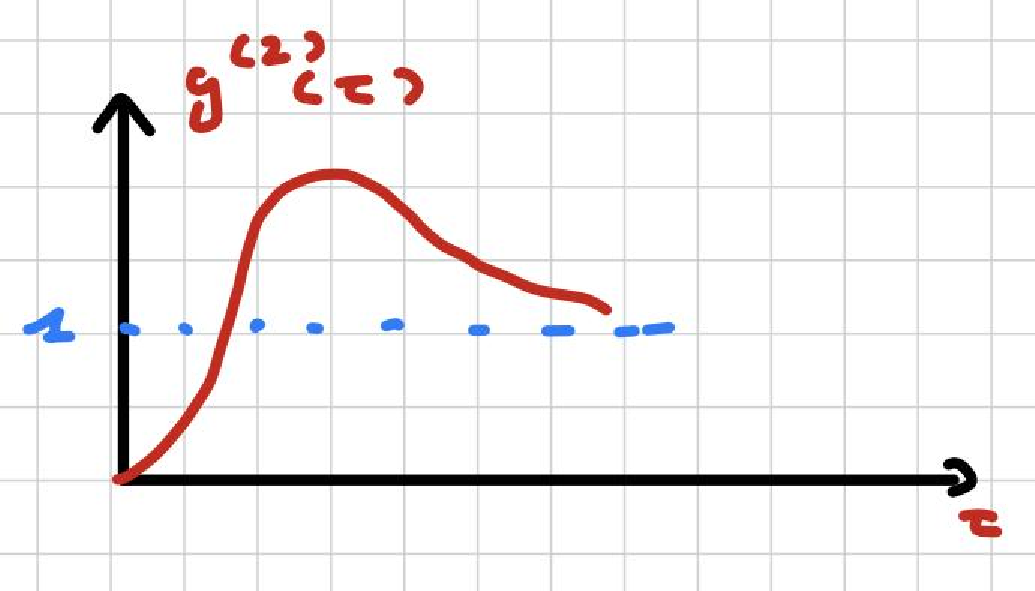
\includegraphics[width=0.6\linewidth]{images_in_pdf/10-/Grafico_56.pdf}
    \end{figure}
    \[
    g^{(2)}(0)<g^{(2)}(\tau), \qquad g^{(2)}(0)<1.
    \]
\end{enumerate}

\calloutwarn{Note that sub-poissonian light is also a clear signature of the quantum nature of light. However, photon antibunching and sub-poissonian statistics \textbf{are distinct nonclassical effects}: they may occur together, but one can also appear without the other.}

\subsection{Experimental demonstration of photon antibunching}
The first experimental demonstration of photon antibunching was provided by Kimble and coworkers:
\begin{itemize}
    \item They sent a dilute beam of sodium atoms along a collimated stream, so that only a very small number of atoms contributed to the fluorescence at any given time;
    \item The atoms were excited by a light beam, and each atom could emit a photon;
    \item The emitted photons were collected by a microscope system;
    \item The light passed through additional optics and a beam splitter, and each output reached a photomultiplier tube;
    \item Each output was amplified and sent through a discriminator;
    \item Finally, the signals were sent to coincidence electronics, one channel providing the start and the other the stop.
\end{itemize}

\calloutwarn{%
    Notice that in a discharge lamp the light is emitted by millions of atoms, each one statistically independent, and this leads to bunched thermal light. In this experiment, instead, \emph{at any given time only one or a few atoms effectively contribute to the fluorescence}, which makes antibunching observable. 
}
\begin{figure}[H]
    \centering
    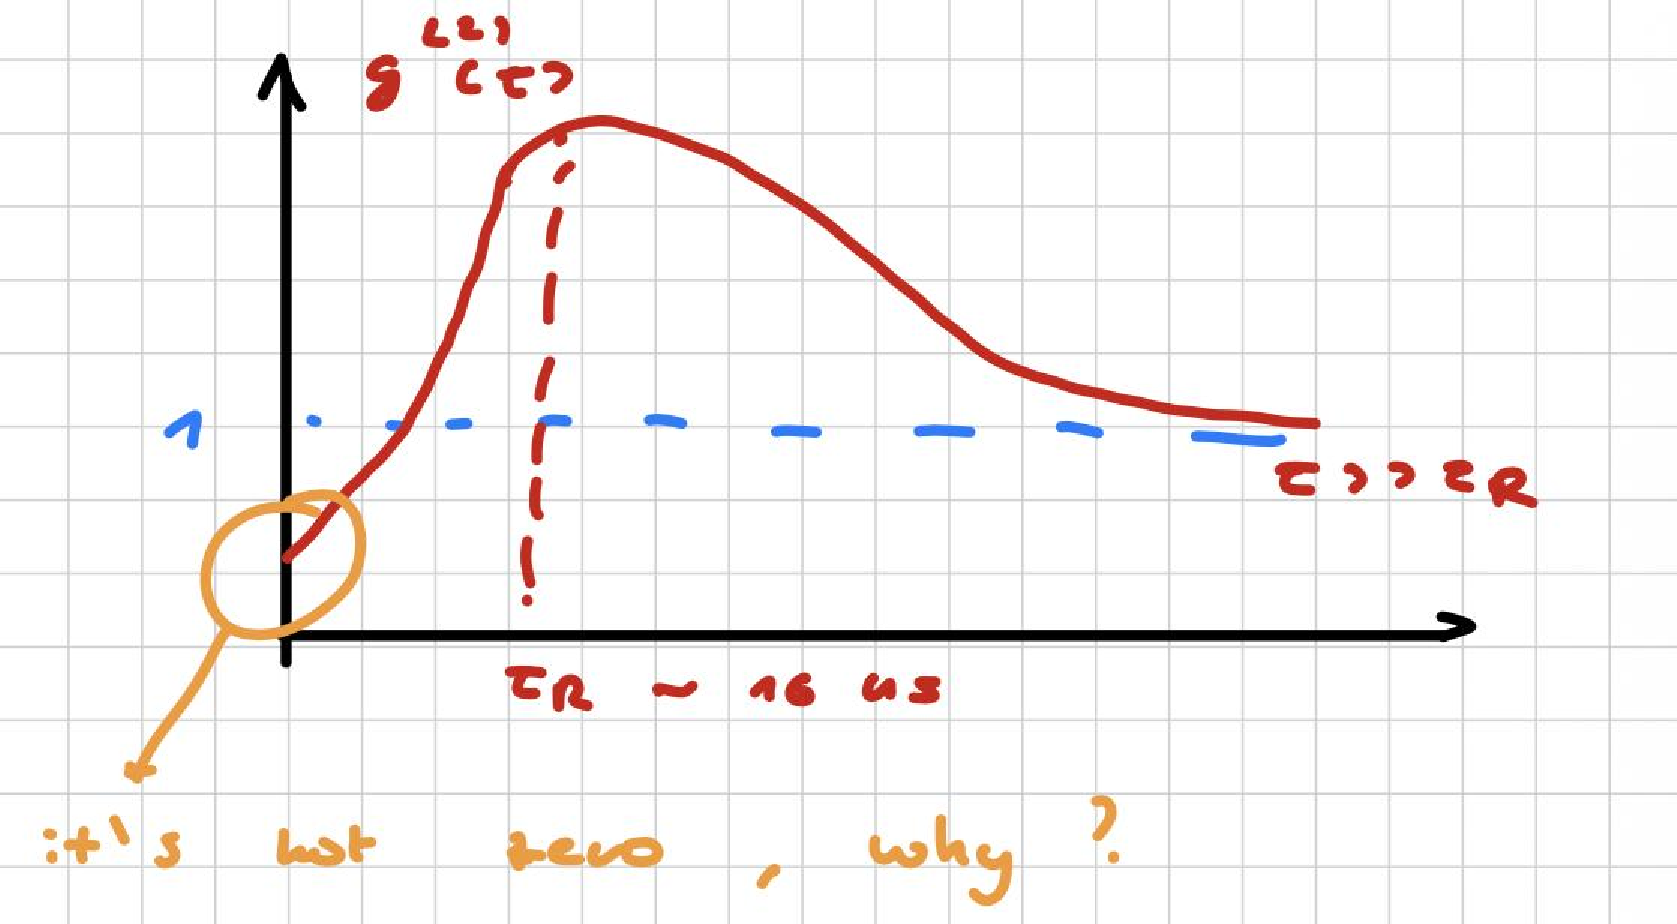
\includegraphics[width=0.6\linewidth]{images_in_pdf/10-/Grafico_57.pdf}
\end{figure}

The observed behavior is:
\begin{itemize}
    \item Ideally, one expects $g^{(2)}(0)=0$. Experimentally, the value is not exactly zero because of detector dark counts, background light, finite time resolution, and the possibility of accidental coincidences.
    \item Then $g^{(2)}(\tau)$ rises on a time scale comparable to the radiative lifetime of the atomic ensemble, $\tau_R \approx 16\,\mathrm{ns}$.
    \item For $\tau \gg \tau_R$, the correlation function decreases toward unity:
    \[
    g^{(2)}(\tau)\to 1.
    \]
\end{itemize}

\hl{This was the first experimental evidence of single-photon emission from a single atom and of anti-bunched light}.

Here a table to sum up the different types of light is provided:

\begin{table}[H]
\centering
\begin{tabular}{@{}ccc@{}}
\toprule
\textbf{Type}         & \textbf{Second order correlation function}                    & \textbf{Source}    \\ \midrule
\textit{Coherent}     & $g^{(2)}(\tau) = 1, \hspace{1ex}\forall \, \tau$ & Classical coherent \\[0.75ex]
\textit{Bunched}      & $g^{(2)}(\tau) < g^{(2)}(0)$                                  & Classical          \\[0.75ex]
\textit{Anti-bunched} & $g^{(2)}(\tau) > g^{(2)}(0)$                                  & Not-classical      \\ \bottomrule
\end{tabular}
\end{table}

\subsection{Single-photon sources}
Single-photon sources must satisfy two fundamental requirements:
\begin{itemize}
    \item the ability to isolate individual emitting species;
    \item the possibility to control the rate at which photons are emitted.
\end{itemize}
To realize such a source, one considers the emission of a single photon in response to an optical or electrical trigger. Let us select an emitting species and examine its energy-level structure.
\begin{figure}[H]
    \centering
    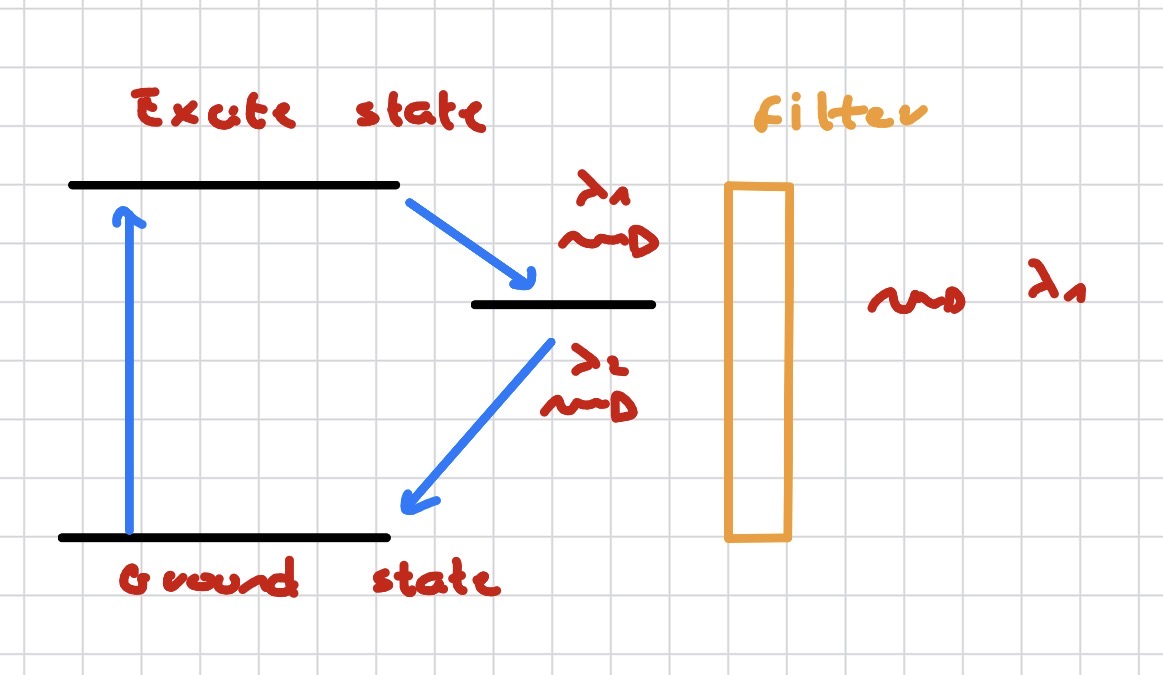
\includegraphics[width=0.6\linewidth]{images_in_png/Grafico_58.jpg}
\end{figure}
The ground state is first excited to a higher-energy state. During relaxation, the system may pass through intermediate states, which can emit photons with different wavelengths $\lambda_1,\lambda_2,\dots$. By inserting suitable optical filters, one can select a specific wavelength and reject the others. In this way, \hl{an optical or electrical pulse acts as a trigger that promotes the electron to an excited state, and the emitter releases one photon after a characteristic radiative lifetime $\tau_R$} for each excitation cycle. The time between two trigger pulses is
\[
T=\frac{1}{f_T},
\]
where $f_T$ is the trigger repetition rate.
\begin{figure}[H]
    \centering
    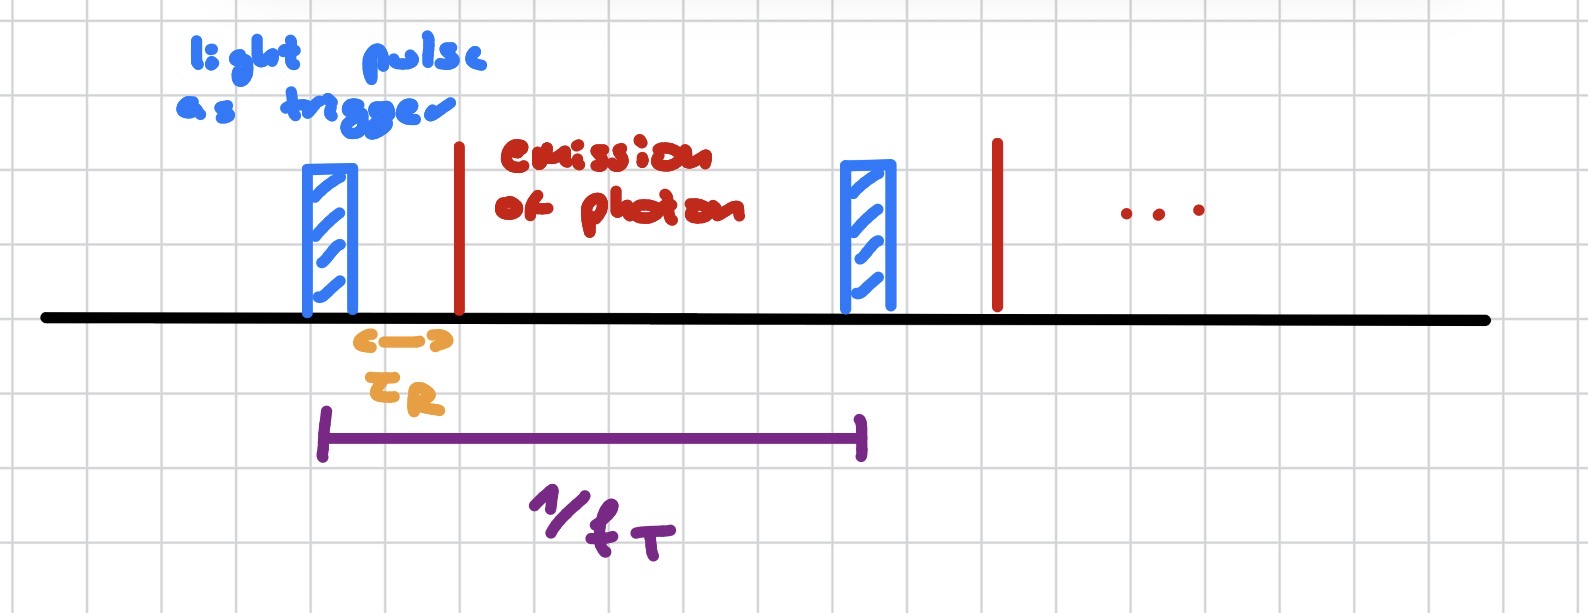
\includegraphics[width=0.6\linewidth]{images_in_png/Grafico_59.jpg}
\end{figure}
No new photon can be emitted until the next trigger pulse arrives.

If
\[
\frac{1}{f_T} = T >\tau_R,
\]
the trigger controls the temporal separation between successive emission events, and the source can exhibit anti-bunched light.

The fluorescence process remains probabilistic, so the photon stream is not perfectly regular. However, the \hl{probability of emitting two photons within a time interval much shorter than $\tau_R$ is very small}, which implies
\[
g^{(2)}(0)\approx 0.
\]

\calloutinfo{%
The use of solid-state emitters instead of atoms is extremely attractive because they are fixed in the lattice and can therefore be integrated into practical devices. Moreover, quantum confinement leads to discrete energy levels, so these nanostructures behave as \textit{artificial atoms}. In a simple confinement picture, the energy levels scale approximately as
\[
E_n \propto \frac{n^2}{L^2},
\]
so that by changing the size of the nanostructure one can select different emission wavelengths for different physical applications.
}

\subsection{Spectroscopy of single semiconductor nanocrystals}
By means of \textbf{molecular beam epitaxy (MBE)} one can fabricate ensembles of nanostructures that are not perfectly identical. They differ in shape, size, defects, surface states, chemical composition, and impurity content. All these factors affect the energy levels $E_n$ and the emission properties. \hl{What is measured experimentally in an ensemble is therefore an average over many different objects}, which produces a large \textbf{inhomogeneous broadening}.

\question{Can we measure the spectra of individual low-dimensional objects?}{
Yes. The first experiments of this kind were performed using optical spectroscopy with high spatial resolution.}

\subsubsection{Potential limitations}

Quantum confinement becomes relevant when the characteristic size of the nanostructure is comparable to the exciton\footnote{An exciton is a bound state of an electron and a hole interacting through the Coulomb potential.} Bohr radius, which is typically of the order of $\sim 10\,\mathrm{nm}$.

However, spatial resolution is limited by diffraction. According to the \textbf{Rayleigh criterion}, two point sources are distinguishable if their separation is at least of the order of the distance between the center of the Airy disk and its first minimum:
\[
d \gtrsim 0.61\,\frac{\lambda}{\mathrm{NA}},
\]
where $\mathrm{NA}$ is the numerical aperture of the objective. 
\calloutwarn{%
    For a common microscope objective, this gives a resolution limit of the order of $10^2\,\mathrm{nm}$, which is much larger than the typical size of a quantum dot.
}
\textbf{But} we are not trying to image the true size of the object itself; instead, \hl{we just want to detect the luminescence signal emitted by a single quantum dot and distinguish it from all other signals}. The following conditions are therefore required:
\begin{enumerate}
    \item the density of objects must be low, so that the \hl{distance between them is larger than the diffraction-limited resolution};
    \item parasitic light sources must be suppressed;
    \item the spatial resolution and image quality must be as high as possible;
    \item the emitted photons must be collected efficiently, which requires a high quantum efficiency $\eta$.
\end{enumerate}
If we take a spot of \qty{200}{\micro\meter}, we expect roughly $10^7$ quantum dots and therefore a broad emission spectrum. If instead we achieve a spot of \qty{200}{\nano\meter}, we can isolate a few emitters and observe sharp lines, leading to spatially resolved photoluminescence from a single quantum dot. 

To achieve this, we need:
\begin{itemize}
    \item a microscope for spatial resolution operating near the diffraction limit;
    \item a spectroscopic system for spectral resolution. The sample is excited by a laser beam inside a cryogenic device, and the emitted photons are collected in an \textbf{epifluorescence} geometry, meaning that excitation and collection occur along the same optical path. A \textbf{grating} provides spectral dispersion, while filters are used to select specific wavelengths.
\end{itemize}
\textbf{Scanning technique (confocal effect):}

To augment our resolution, we can use two lenses and an optical axis. Suppose a source is placed on the optical axis and its light is collected by both lenses and sent to a spectrometer. If a pinhole is inserted between the lenses, the spatial resolution improves because light coming from sources away from the optical axis is blocked by the iris (i.e., the pinhole along with the optical axis). In this way, out-of-focus contributions are strongly suppressed.
\begin{figure}[H]
    \centering
    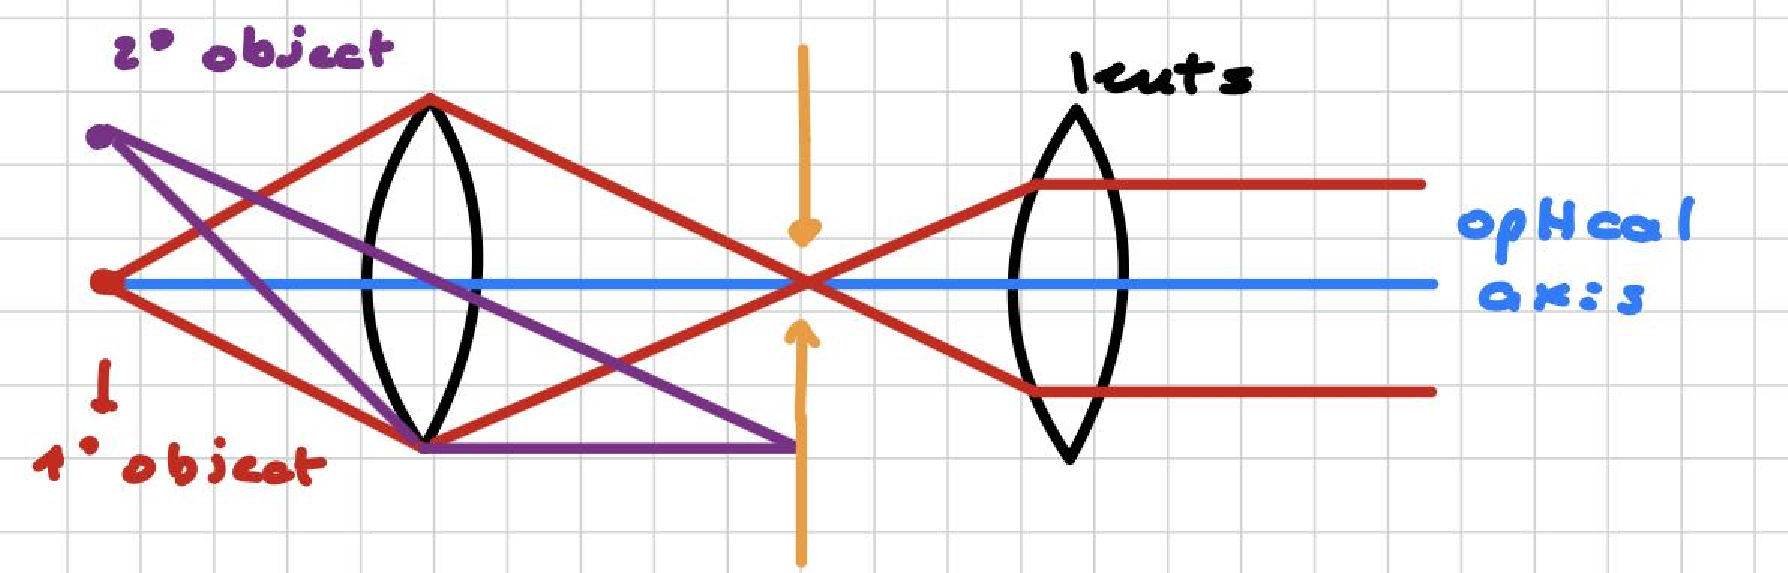
\includegraphics[width=0.6\linewidth]{images_in_pdf/10-/Grafico_60.pdf}
\end{figure}

Scanning is achieved either by moving the sample, which is glued on an $x,y,z$ stage, or by moving the excitation spot using piezo-positioned mirrors. The sample is illuminated by a laser beam, and for each position the emission spectrum is measured. In this way, one reconstructs a three-dimensional map of the material emission. The emitted light is collected along the same path (epifluorescence), passes through a dichroic mirror\footnote{A dichroic mirror is a mirror that reflects certain wavelengths while transmitting others.} and the optical system described above, and is then directed toward a beam splitter.
The two outputs (the reflected beam and the fluorescence one) go directly in two detectors and can be used either to measure the fluorescence lifetime with time-correlated single-photon counting or to study light statistics through the second-order correlation function.
\begin{figure}[H]
    \centering
    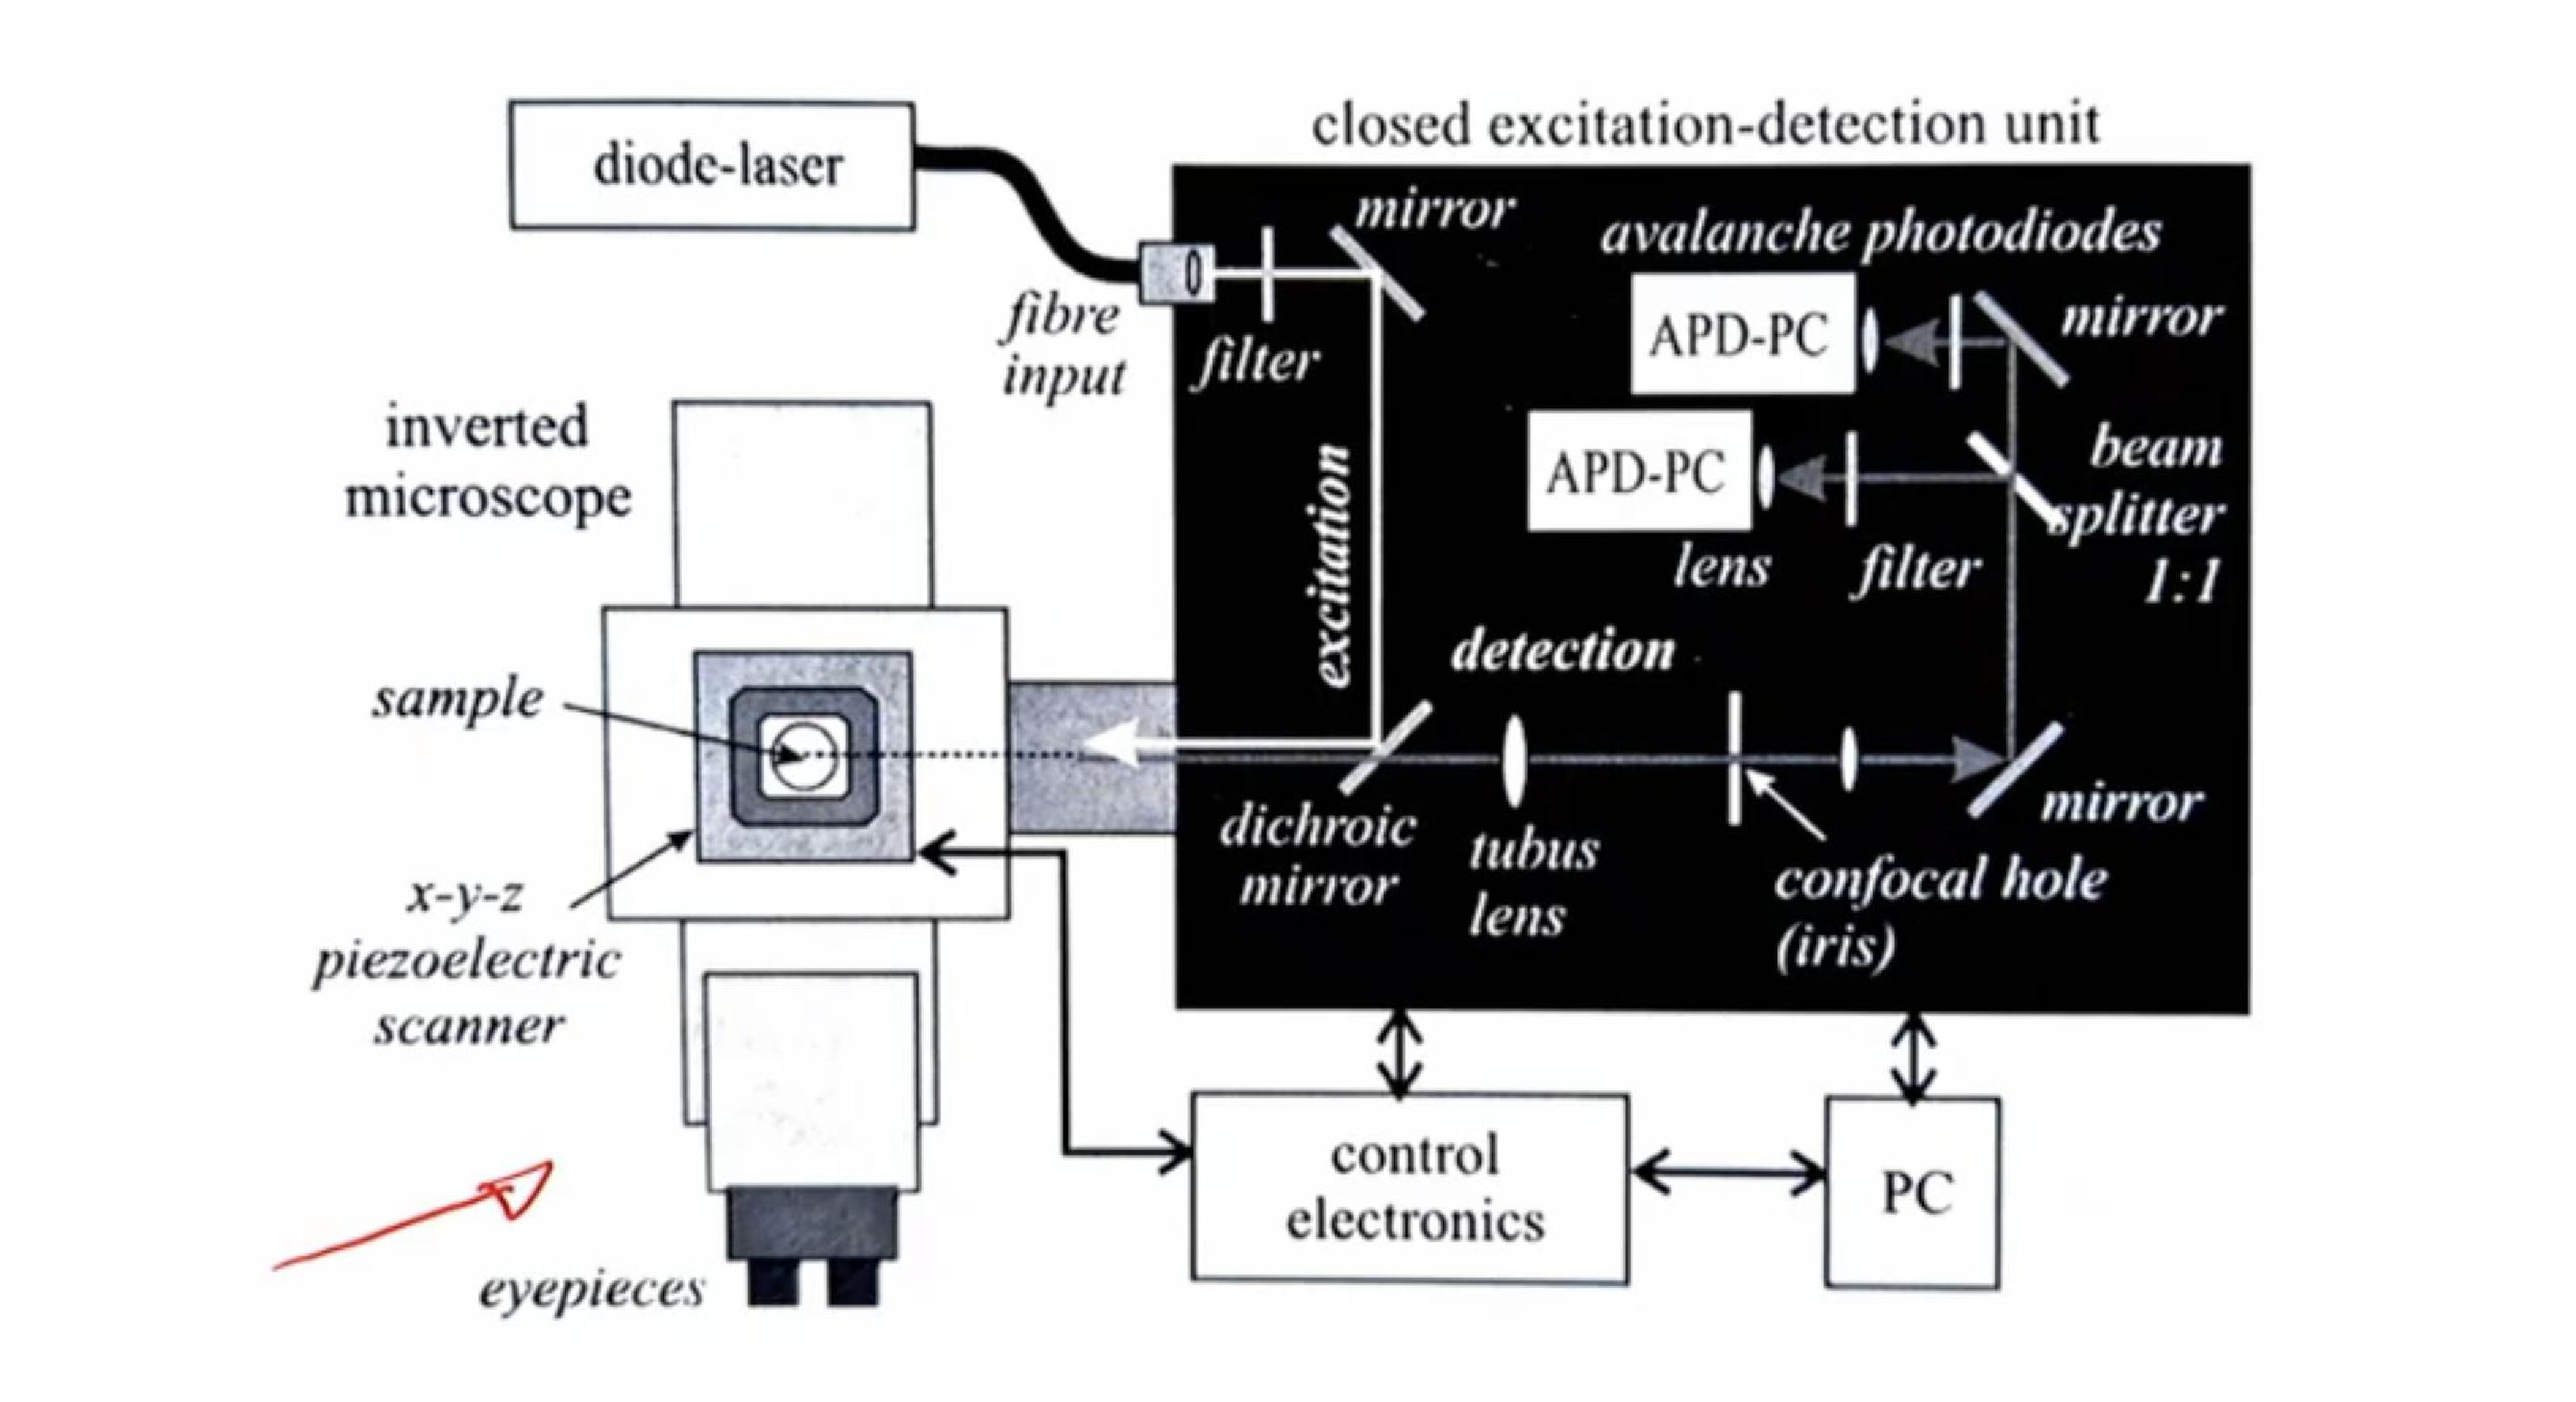
\includegraphics[width=0.6\linewidth]{images_in_pdf/10-/Grafico_61.pdf}
\end{figure}

Compared with an ensemble, the photoluminescence of individual nanocrystals always shows much narrower spectral lines, whose width is ultimately limited by the radiative lifetime $\tau_R$, by means of the energy-time uncertainty principle (Eqn.~\ref{eqn:6-energy-time-uncertainty}). In the lifetime-limited case, the linewidth scales as
\[
\Delta E \sim \frac{\hbar}{\tau_R},
\]

so for $\tau_R \approx \qty{1}{\nano\second}$ the spectral width is typically of the order of $\unit{\micro\electronvolt}$.

\subsubsection{Example: QD with InAs}
\begin{figure}[H]
    \centering
    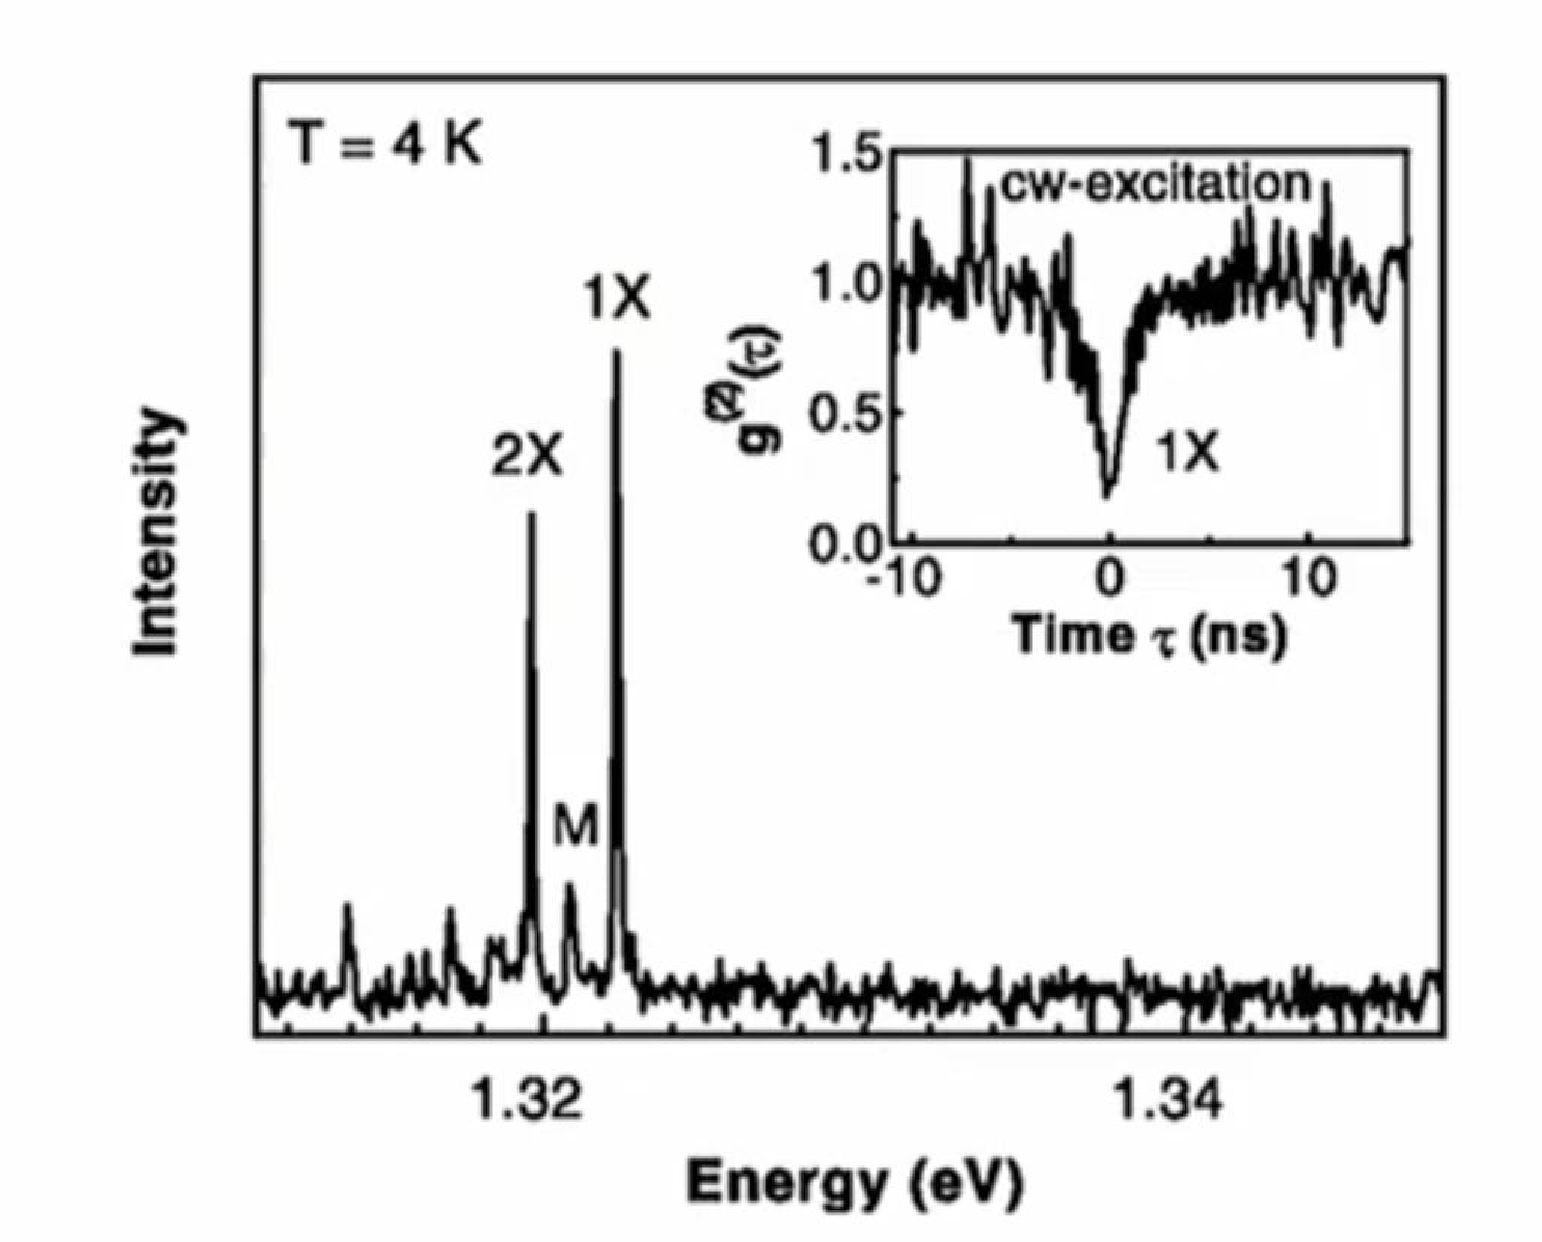
\includegraphics[width=0.6\linewidth]{images_in_pdf/10-/Grafico_62.pdf}
\end{figure}

The peak labeled $1X$ corresponds to exciton recombination, while $2X$ corresponds to bi-exciton recombination. The second-order correlation function is close to zero, with a typical experimental value of about $g^{(2)}(0)\approx 0.2$, which is a clear signature of an anti-bunched light source. 

\question{But why is it not exactly zero?}{%
The answer is that the detector time response, about \qty{0.4}{\nano\second}, must be compared with the radiative lifetime of about \qty{2.2}{\nano\second}. There is therefore a nonzero probability of detecting two events within a time interval that the detector cannot fully resolve (i.e. both events are considered at $t=0$). This is why the time jitter of the detector is so important.
}

We can illustrate this with a numerical example:
\begin{figure}[H]
    \centering
    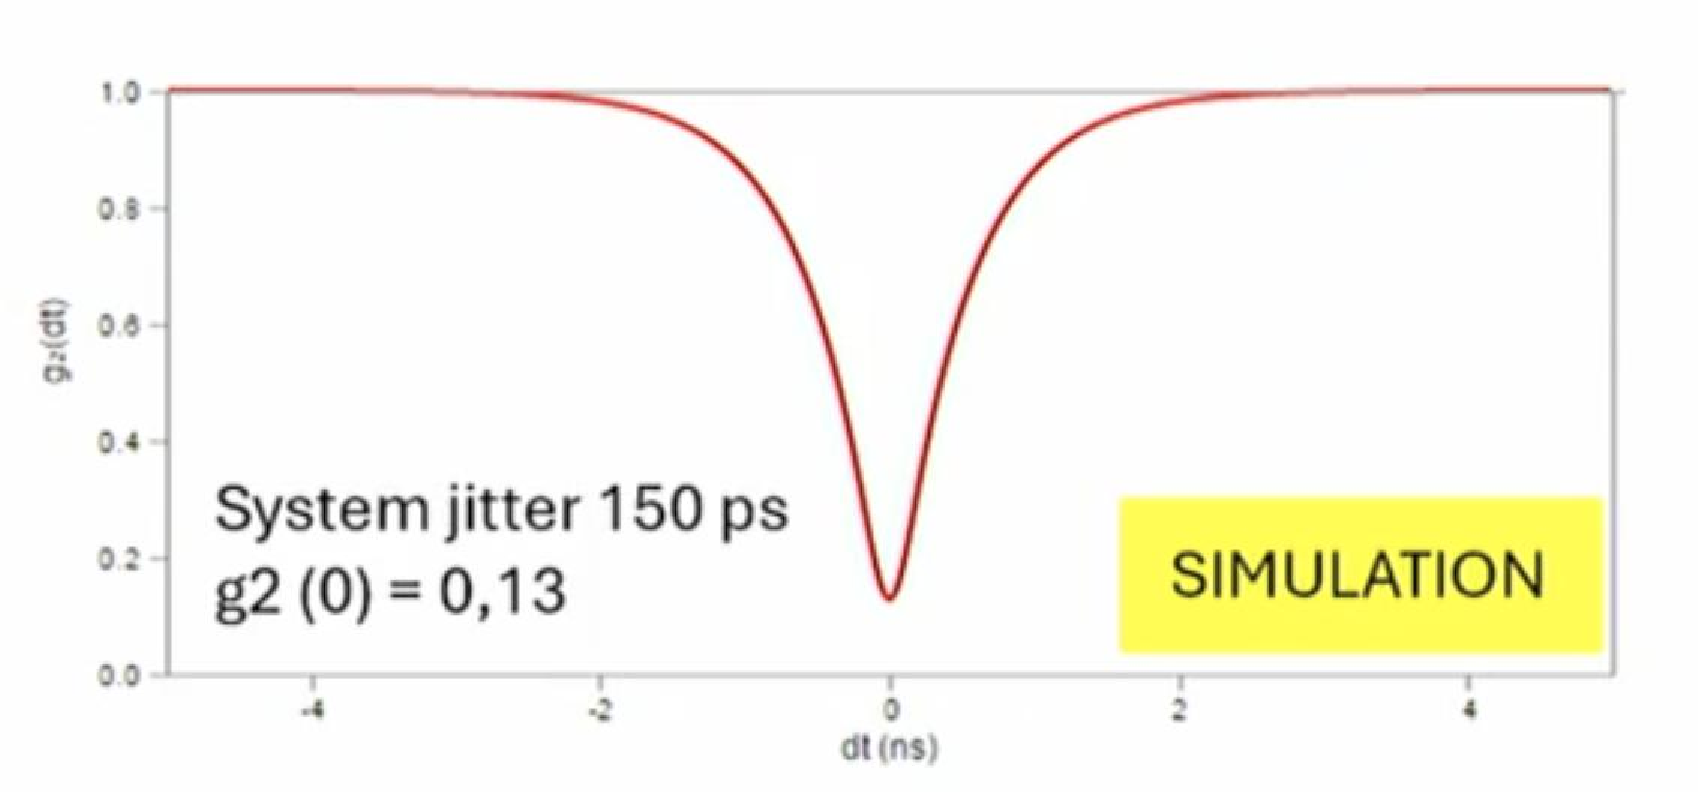
\includegraphics[width=0.6\linewidth]{images_in_pdf/10-/Grafico_63.pdf}
\end{figure}

\begin{figure}[H]
    \centering
    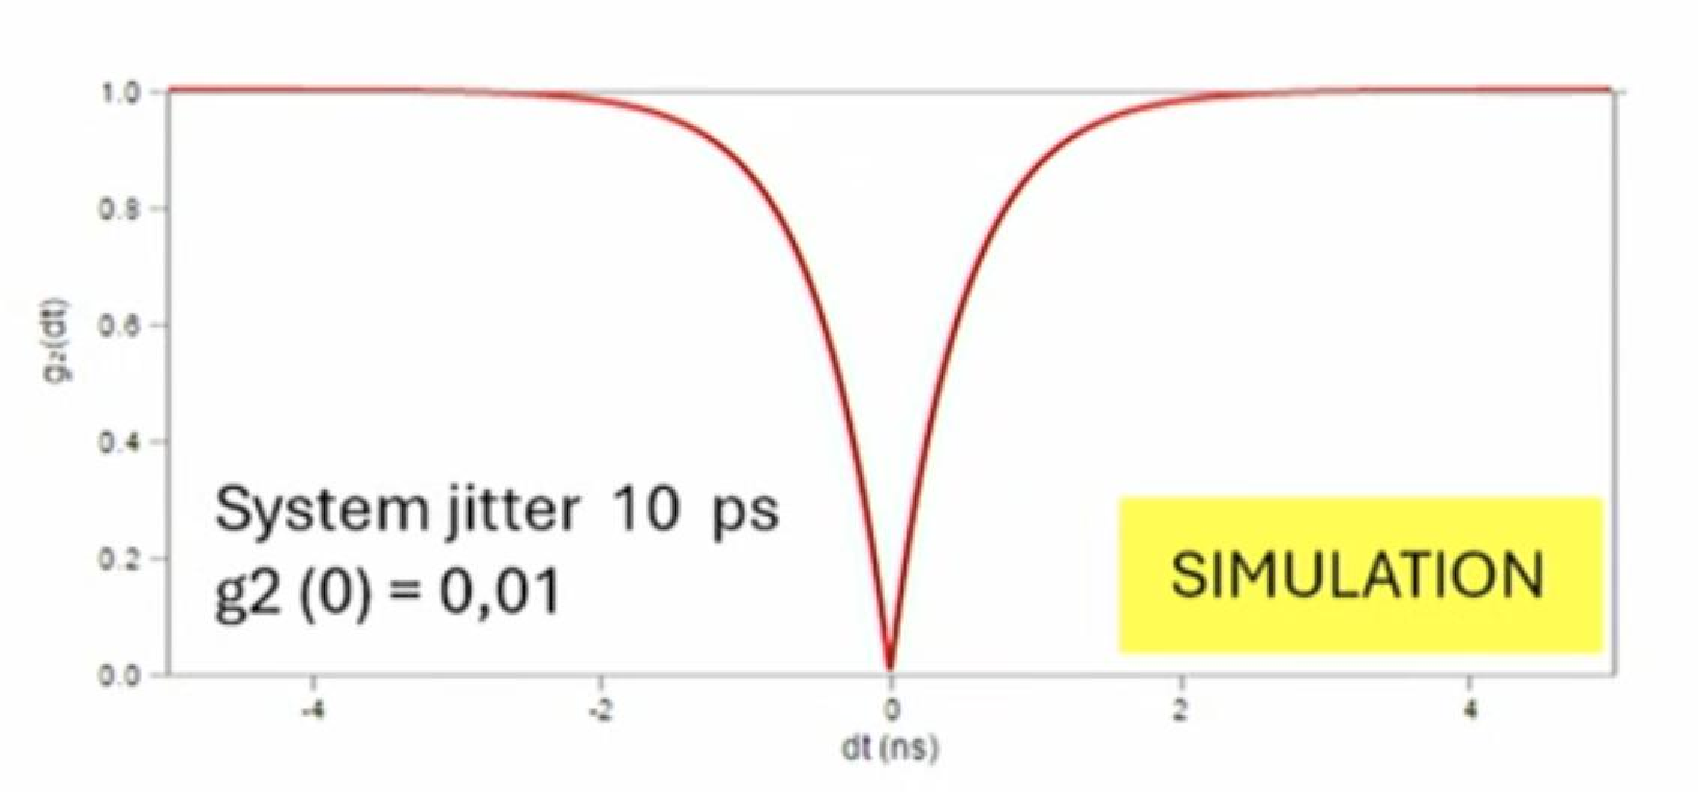
\includegraphics[width=0.6\linewidth]{images_in_pdf/10-/Grafico_64.pdf}
\end{figure}

If the time jitter of the detector is reduced, the measured value of $g^{(2)}(0)$ approaches zero.
